
\documentclass[12pt]{report}

\usepackage{setspace}
\onehalfspacing %doublespace %

\usepackage{amssymb,amsmath,amsthm}

\setlength{\intextsep}{1ex}

%\usepackage[dvips]{graphicx}
\usepackage{graphicx}
\include{epstopdf}
\renewcommand{\qedsymbol}{\rule{0.4em}{0.4em}}
\usepackage{tabularx}

\usepackage[a4paper,bindingoffset=25mm,%
            left=0mm,right=15mm,top=15mm,bottom=15mm,%
            footskip=5mm]{geometry}

\usepackage{lipsum}  


\usepackage[english]{babel}
\usepackage{float}
\setlength{\intextsep}{1ex}
\usepackage[shortlabels]{enumitem}
\usepackage{multirow}
\usepackage[font={small}]{caption}
\usepackage{nameref}

\usepackage[justification=centering]{caption}
\usepackage{caption,subcaption}
\usepackage[toc,page]{appendix}
\usepackage{amsmath}
\usepackage{color}
\usepackage[parfill]{parskip}
\usepackage{listings}
\definecolor{dkgreen}{rgb}{0,0.6,0}
\definecolor{gray}{rgb}{0.5,0.5,0.5}
\definecolor{darkgray}{rgb}{.4,.4,.4}
\definecolor{purple}{rgb}{0.65, 0.12, 0.82}
\definecolor{mauve}{rgb}{0.58,0,0.82}

\lstset{frame=tb,
language=Python,
aboveskip=3mm,
 belowskip=3mm,
 showstringspaces=false,
columns=flexible,
 basicstyle={\small\ttfamily},
 numbers=none,
numberstyle=\tiny\color{gray},
 keywordstyle=\color{blue},
 commentstyle=\color{dkgreen},
stringstyle=\color{mauve},
 breaklines=true,
 breakatwhitespace=true,
 tabsize=3
}


\setlength{\parskip}{10pt}
\setlength{\parindent}{0pt}

\renewcommand{\bibname}{References}


\setlength\parindent{0pt}
\setlength{\unitlength}{1cm} 


\begin{document}

\begin{titlepage}
\centering

\begin{figure}[H]
\centering

\includegraphics[width=0.4\textwidth]{MAK_Logo2_png.png}%
\end{figure}


\textsc{}

\vspace{\stretch{0.1}}

{\huge \textsc{Design of a Deep Learning based Pothole Detection System}  \\}
\rule{3in}{0.4pt}

\vspace{\stretch{0.4}}

{\Large\textbf{Walaga Priscilla N Edith}	 \\}
Student ID: 16/U/12253/PS\\ \vspace{2cm}
{\large \textbf{Department of Electrical and Computer Engineering} \\
School of Engineering \\
College of Engineering, Design, Art and Technology}



\vspace{\stretch{0.3}}

{
Supervisor: \textbf{Dr Andrew Katumba}    \\
Co-supervisor: \textbf{Dr Jonathan Serugunda} }

\vspace*{\stretch{0.2}}

% Add date in desired format
December 7, 2020


\vspace*{\stretch{0.2}}
% Add the statement of what the report represents
{
A Report submitted in partial fulfillment of the requirements for the \\ \textbf{ Degree of Bachelor of Science in Computer Engineering} \\ at Makerere University. }


\end{titlepage}



%\maketitle
				
%\beforeabstract %\input{abstract} 



\section*{Declaration}

I Walaga Priscilla N Edith hereby declare that the material submitted in this  report has been written and complied by me to the best of my ability and has not been submitted to any other University before for an award in the degree of Bachelor of Science in Computer Engineering. 

Academic Integrity Pledge

I HAVE ABIDED BY THE MAKERERE UNIVERSITY ACADEMIC INTEGRITY POLICY ON THIS ASSIGNMENT.



Signature…………………………. Date……………………… 

Walaga Priscilla N Edith

APPROVAL 

This report has been submitted with the approval and under the supervision of the following supervisors.


Main Supervisor 


Signature…………………………. Date……………………… 

Dr Andrew Katumba



Co Supervisor 


Signature…………………………. Date……………………… 

Dr Jonathan Serugunda



\newpage


\section*{Dedication}

%\vspace{2cm}

I dedicate this report to my loving family for the support rendered to me, my supervisors and all people who have supported me.




\newpage

\section*{Acknowledgments}

To begin with, I would like thank the Almighty God for enabling me complete my course at Makerere University. I also extend my sincere gratitude to the Department of Electrical and Computer engineering, the College, and Makerere University for the careful and precious guidance, training and a good learning environment which were of value throughout my study period.

I take this opportunity to convey my special thanks to Dr Andrew Katumba, Dr.Jonathan Serugunda  for their guidance, support and knowledge during my final year project despite their busy schedules.

Special thanks go to my project partner, Titus Weikama, for the cooperation, and assistance received throughout the project period.







\newpage



\section*{Abstract}


With an increasing number of  potholes on the roads that take a while before they are repaired, their adverse effects like accidents,traffic jam, flooding during the rainy season and damage to motor vehicles keep affecting road users. However automating the process of the location and detection of these potholes can cut down the amount of time it takes for these potholes to be repaired from when they are first located.

This report therefore presents the Design of a Deep Learning  Based Pothole Detection System which involves a deep analysis on the use of machine learning and Convolutional Neural Networks in computer vision and object detection. This study will involve training a machine learning model with pothole dataset and later developing a model that can detect the presence of these potholes on the roads.

Data collection was done by taking picctures in form of videos of different roads inside a moving vehicle by use of a mobile phone placed on a car windscreen. A total of 836 images was collected, the images were resized and labelled by drawing bounding boxes around the potholes in the images. The images were then converted to a format compatible with the training algorithm, the COCO dataset format. For training the EfficientDet algorithm was used which is a high accuracy, high efficiency algorithm with each layer images go through different kkinds of optimization till the box layer.

Model training using the efficientdet algorithm was succesful and a machine learning model that detects potholes with an Average Precison of 0.52515274 was developed. A pothole dataset of 836 images was  collected and is stored in a database.



\newpage

\tableofcontents

\newpage

\listoffigures

\newpage

\listoftables

\newpage



\section*{List of Abbreviations}

\begin{tabular}{p{3cm} l}
	AI & Artificial Intelligence\\
API & Application Programming Interface\\
CNN & Convolutional Neural Network\\ 
COCO & Common Objects in Context\\ 
CPU & Central Processing Unit \\
CSV & Comma Seperated Values \\
DL & Deep Learning\\
FLOPS & Floating Point Operations Per Second \\
FN & False Negative\\
FP & False Positive\\
GPS & Global Positioning System\\
GPU & Graphics Processing Unit \\
IoU & Intersection over Union \\
ML & Machine Learning \\
RAM & Random Access Memory \\
ROI & Region Of Interest \\
SSD & Single Shot MultiBox Detector \\
SVM & Support Vector Machine \\
TF & TensorFlow Records \\
TP & True Positive\\
TPU & Tensor Processing Units \\
UNIX & Uniplexed Information Computing System \\
USB & Universal Serial Bus \\
YOLO & You Only Live Once \\


\end{tabular}









\chapter{Introduction}

\section{Background}

Uganda has a total road network of 146,000Km of which 14.8\%  are national roads. These are under the management of Uganda National Road Authority. Of these, 22.2\% are paved while 77.8\% are unpaved. National roads host 80\% of the average daily road traffic on the road network and are a strong driver for social-economic development. Inorder to sustain this development, it is important that these roads are adequately maintained\cite{Roads}.

However these maintenance works happen after very long periods of time and this has led to continued depletion of these roads by potholes. Majority of the national roads are made-up of atleast 3-7 potholes and this has become a major danger to both vehicle owners as they cause damage to their vehicles and also to the pedestrians. Road maintenance works take a lengthy time due to the steps that are involved from when a pothole is first known about/ detected to the final stage of actual repair.




\section{Problem Statement}

The status of potholes and their repair is the issue of being able to detect and locate the potholes in a timely manner. The repair process takes a long time as some roads are located in remote areas and it requires time and money to travel to these areas and locate the exact area that needs repair. Repair is not effected immediately even after the detection process but rather more planning is needed until the final repair stage. When not repaired they cause accidents to the road users, damage vehicles and when they continue to increase in size some become mosquito breeding areas during the rainy season and most of all they lead to accelerated aging of roads. 
Currently each municipal is assigned an Engineer whose responsible for all the roads in that area.Quartely the engineer carries  out a survey on the roads in the municipal and notes down those that need repair.After identifying these roads, they make a plan for repair and maintenance and also a budget. This budget and plan is sent to the Uganda Road Fund which provides funds for road repair and maintenance. The plan and budget are approved after being prsented to the Minister incharge of road approval. After all this funds are finally recieved and road repair takes place. This is a very timely process that can be made shorter by automating the process of pothole detection\cite{Road--Fund}


\section{Justification}
Automation of pothole detection will aid Engineers maintain roads better because the whole detection process will have been made easier and will be readily available in the form of images stored in a database. From this there will be proper and timely planning for road repairs hence reducing the adverse effects caused by the continual existence of these potholes like accidents, flooding during the rainy season, traffic jam and damage to cars. For the government, automation of the detection process will reduce on the costs spent in travelling to the different districts to carry out these road surveys as the pothole information will be avaliable on a database. With this automated system in place in the long run,the shelf--life of roads will increase due to their timely repair/ maintenance.




\section{Aims and Objectives}

The main aim of the research project was to design a deep learning  pothole detection system to determine the presence and predict the severity of potholes.

The specific objectives of the research were:

\begin{itemize}[topsep=0pt]

\item To  create a dataset of pothole images stored in a database.

\item To  train a machine learning  model using Convolutional Neural Network that detects potholes.

\item Evaluation of the performance of the machine learning model  that detects potholes.


\end{itemize}









\section{Contributions of the Project}

The following major contributions have been accomplished during the course of this research:

\begin{enumerate}[topsep=0pt]

\item Built a dataset of pothole images.

\item Trained a machine learning model that detects potholes.

\item Evaluated a machine learning model that detects potholes


\end{enumerate}






\section{Organization of the Report}

This report has five chapters,

\textbf {Chapter One} is the Introduction that gives a background of the project, it then looks at the problem statement and highlights the major objectives for carrying out this research and also indicates the contributions of this research.

\textbf {Chapter Two} is the Literature Review that contains literature about the project,describing different techniques used in the project,similar workdone by others and the different techniques they used to do this work.
  of the technologies used in this project.

\textbf {Chapter Three} is the Methodology that contains all the exact steps followed to carry out each objective, data collection, data-pre-processing, model training and evaluation of the model. It also has a section of all the technologies used in the project.

\textbf{Chapter Four} is the Results that contains all the results obtained from the methodolgy, in form of images, graphs and other parameters.

\textbf{Chapter Five} is the last chapter that contains recommendations on the project and the future work to be done and the conclusion.
 

% Describe what each chapter discusses.















\chapter{Literature Review}
% Usually Literature Review

\section{Introduction}
This chapter provides the detailed literature about Machine learning, Object detection and Convolutional Neural Networks  and how it has been used in relation to pothole detection as well as related literature associated with this project.

% Start with an introduction
\section{Artificial Intelligence}
Arficical Intelligence refers to the simulation of human intelligence in machines that are programmed to think like humans and mimic their actions. The ideal characteristic of AI is its ability to rationalize and take actions that have the best chance of achieving a specific goal. AI is based on the principle that human intelligence can be defined in a way that a machine can easily mimic it and execute tasks from the most simple to those that are even more complex.The goals of AI include learning, reasoning, and perception and it is being used across different industries like finance and healthcare\cite{AI}. 

\begin{figure}[H]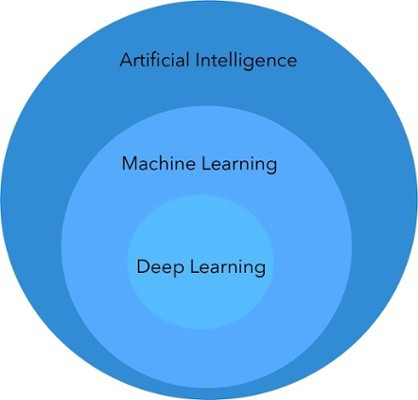
\includegraphics[scale=0.7]{ML.jpeg}\centering\caption{Relationship between AI, ML and DL \cite{Difference}} \label{fig:AI, ML, DL} \end{figure}


\section{Machine Learning}
Machine Learning is an application of artificial intelligence that provides systems the ability to automatically learn and improve from experience without being programmed.Machine learning relies on features that are considered important within the dataset. A dataset is simply input data developed from the sampled area of study in this case pothole images is the dataset. Machine learning is generally split into: supervised learning and unsupervised learning. \cite{Machine--Learning}. 

\subsection{Supervised Learning}
Supervised Learning teaches a machine by example. During the training for supervised learning, machines are exposed to large amounts of labelled data like images of handwritten figures annotated to indicate which number they correspond to. If given sufficient examples, a supervised-learning system would learn to recognize the clusters of pixels and shapes associated with each number and eventually be able to recognize handwritten numbers and also reliably distinguish between the different numbers\cite{Supervised}.
However, training these systems typically requires huge amounts of labelled data, with some systems requiringto be exposed to  millions of examples to master a task. Some popular examples of supervised machine learning algorithms ar\cite{Super}:

\begin{itemize}[topsep=0pt]

\item Classification-- A classification problem is when the output variable is a category like, red or blue or disease and no disease.

\item Regression-- A regression problem is when the output variable is a real value such as "dollars" or weight.

\end{itemize}
Some popular examples of supervised machine learning algorithms include;  linear regression and Random forest.

\subsection{Unsupervised Learning}
In unsupervised learning, users do not need to supervise the model, it allows the model to work on its own to discover patterns and information that was previously undetected and it deals with mainly unlabelled data. Unsupervised Learning algorithms allow users to perform complex processing tasks compared to supervised learning\cite{Super}.Types of unsupervised learning include;

\begin{itemize}[topsep=0pt]

\item Clustering-- This is where you want to discover the inherent groupings in the data, such as grouping customers by purchasing behavior.

\item Association-- An association rule learning problem is where you want to discover rules that describe large portions of data, such as people that buy X also tend to buy Y.

\end{itemize}
Some popular examples of unsupervised learning algorithms include; k-learning and Apriori algorithm\cite{Unsupervised}.

\subsection{Semi-supervised}
This approach mixes supervised and unsupervised learning.This technique relies upon using a small amount of labelled data and a large amount of unlabelled data to train systems. The labelled data is used to partially train a machine-learning model and then that partially trained model is used to label the unlabelled data, a process called pseudo-labelling. The model is then trained on the resulting mix of the labelled and pseudo-labelled data\cite{Supervised}.


\section{Computer Vision}
Computer vision is a science field that deaals with how computers can gain high-level understanding from digital images or videos. It seeks to understand and automate tasks that human visual systems can do.Computer vision tasks follow three processes that excute one after the other\cite{Vision};

\begin{itemize}[topsep=0pt]

\item Image Acquisition- This translates the analog images into digital images, which means it transforms a normal image into binary data. Several tools like webcams, digital cameras are used to build such datasets. Often these raw data are post processed to achieve more efficiency for the next step.

\item Image processing- Some low--level processing is performed on digital images using advanced applied mathematical algorithms or AI image processing algorithms. Information related to the geometric elements of objects in an image is extracted here.

\item Image analysis and understanding- High--level algorithms are applied to the processed data to perform the data's actual analysis and this helps in decison making\cite{Vision}.
\end{itemize}

% Add sections and (sub)subsections as appropriate
\section{Deep Learning}
Deep learning is a subset of machine learning that uses a layered struture of algorithms called neural networks, their design is based on the biological neural network of the human brain. This leads to a process of learning that is more capable than that of standard machine learning models \cite{Deep-Learning}.
Convolutional Neural Networks are a class of neural artificial networks that are currently dominant in computer vision tasks and that's why they are used for this specific project.


\subsection{Convolutional Neural Networks}
Convolutional Neural networks apply deep learning that involves visual study especially image processing of a given sample study. Unlike other image processing technologies CNNs are capable of distinguishing a large number of classes and they require lesser computations due to the sparsely connected neurons and the pooling process\cite{Y.J.Cha}.
CNN's are made up neurons with learnable weights and biases, each neuron receives inputs and takes a weighted sum over them then it passes it through an activation function and gives an output value. CNN's are made of three layers namely\cite{Raghav};

\begin{itemize}[topsep=0pt]

\item The Convolutional Layer is the core building block that does majority of the compuational heavy lifting.It extracts features from an input image, it learns image features by using small squares of the input data.

\item The Activation Layer applies the Recified Linear Unit which applies the recitifier function that increases non-linearity in the neural network.
\item The Pooling Layer reduces the number of parameters when the images are too large. Spatial pooling involves downsampling of features which reduces the dimensionality of each map but retains important information.

\item The Fully Connected Layer invloves flattening, it involves transdorming the pooled feature map matrix into a single column which is then fed to the neural network for processing.

\end{itemize}

\begin{figure}[h!]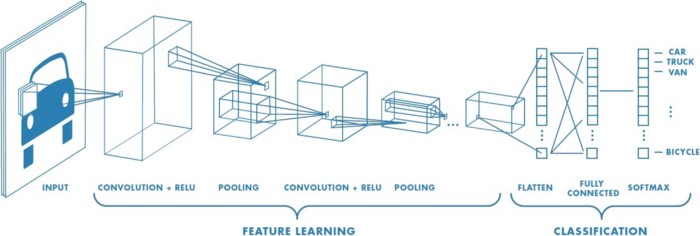
\includegraphics[width=0.9\textwidth]{CNN.jpeg}\caption{Convolutional Neural Network\cite{Raghav}}\label{fig:CNN} \end{figure}%

\section{Road Damage Detection Using Deep Neural Networks with Images Captured Through a Smartphone}

Research on damage detection of road surfaces using image processing techniques has been actively conducted, achieving considerably high detection accuracies. Many studies only focus on the detection of the presence or absence of damage. However, in a real-world
scenario, when the road managers from a governing body need to repair such damage, they need to clearly understand the type of damage in order to take effective action\cite{Neural}.

In this study, we used a state-of-the-art object detection method using convolutional neural networks to train the damage detection model with our dataset, and compared the accuracy and runtime speed on both, using a GPU server and a smartphone. Finally, we demonstrate that the type of damage can be classified into eight types with high accuracy by applying the proposed object detection method.

\subsection{Object Detection System}
In general, for object detection, methods that apply an image classifier to an object detection task have become mainstream; these methods entail varying the size and position of the object in the test image, and then using the classifier to identify the object.
Image processing methods have historically developed at a considerable pace\cite{Neural}. In our study, we primarily focus on four recent object detection systems: the Faster R-CNN\cite{CNN} ,the You Look Only Once (YOLO)\cite{YOLO}  and the Single Shot Multibox Detector (SSD) system\cite{SSD}.

In all these object detection systems, a convolutional feature extractor as a base network is applied to the input image in order to obtain high-level features. The selection of the feature extractor is considerably important because the number of parameters and layers, the type of layers, and other properties directly affect the performance of the detector.Some of these used include:

\begin{enumerate}[topsep=0pt]

\item Inception V2- enable one to increase the depth and breadth of the network without increasing the number of parameters or the computational complexity by introducing so-called inception units..

\item Inception Resnet V2- improves recognition accuracy by combining both residual connections and Inception units effectively.

\item MobileNet- has been shown to achieve an accuracy comparable to VGG-16 on ImageNet with only 1/30th of the computational cost and model size. MobileNet is designed for efficient inference in various mobile vision applications. Its building blocks are depthwise separable convolutions that factorize a standard convolution into a depthwise convolution and a 1 X1 convolution, effectively reducing both the computational cost and number of parameters\cite{Neural}.

\end{enumerate}
 
The SSD using Inception V2 and SSD using MobileNet were used because of  relatively small CPU loads and low memory consumption, even while maintaining high accuracy.

We trained and evaluated the damage detection model using our dataset. Based on the results, in the best-detectable category, we achieved recalls and precisions greater than 75\% with an inference time of 1.5 s on a smartphone. We believe that a simple road inspection method using only a smartphone will be useful in regions where experts and financial resources are lacking. To support
research in this field, we have made the dataset, trained models, source code, and smartphone application publicly available. In the
future, we plan to develop methods that can detect rare types of damage that are uncommon in our dataset\cite{Neural}.




\section{Pothole Detection System Using a Black-box-Camera}
Recently, the resolution of black-box cameras has become sufficiently high for capturing details of a road’s surface. However, detecting potholes using video data has not been developed in the automotive industry, and most proposed models were implemented on desktop computers. Real-time pothole-detection systems using black-box cameras have yet to be tested in the field.

In this paper, we propose a novel pothole-detection system using a commercial black-box camera. The proposed system is mounted on the front windshield of a vehicle and can detect a pothole in real-time. A pothole-detection algorithm is installed on an embedded board in the black-box camera. This algorithm collects information regarding the size of potholes and their location, and this information is  
stored in the black box and then transmitted to a pothole-management server. The proposed pothole-detection algorithm is uniquely designed in consideration of the embedded boards in black-box cameras\cite{Jo}.

\subsection{Proposed Maintenance System}
Pothole information, such as size, location and appearance, is collected by the pothole-detection system using the camera. The collected data is stored in the pothole database, and the pothole-maintenance server uses it for smart pothole maintenance. We developed new software for the pothole-maintenance server based on our previous pothole database system. This software provides various pieces of information about potholes such as their video clips, images, regions, road authorities, route number of a road, driving direction, lane number of the road, type of road, latitude, longitude, collectors, collected date, type of pavement, location, shape, size, and comments\cite{Jo}.

 The pothole’s location is visualized on a digital map using the collected GPS data. Thus, users can easily see the distribution of potholes. Furthermore, the software accurately estimates the costs of pothole maintenance in the selected area. This way,transportation officials can easily and accurately develop road-maintenance policies and strategies with the software. Potholes can then be repaired smartly using the pothole-maintenance system such as our intelligent asphalt repair systems , and pothole information can be extended to other users and services via external connections and OpenAPI\cite{Jo}.

\begin{figure}[H]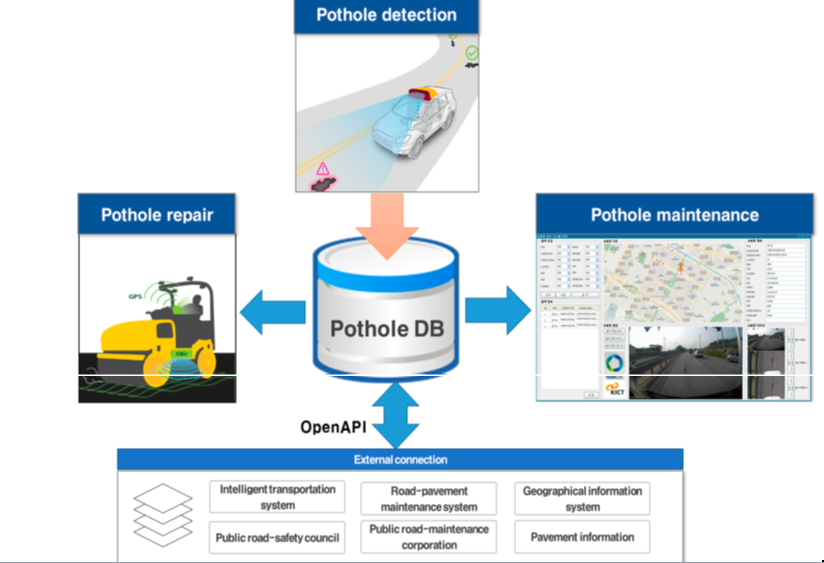
\includegraphics[scale=0.7]{blackbox.png}\centering\caption{Proposed\cite{Jo}} \label{fig:Proposed pothole-maintenance system} \end{figure}%

\subsection{Algorithm}
The proposed pothole-detection algorithm for the black-box camera is divided into three steps: pre-processing, candidate extraction, and cascade detection. First, we perform image cropping, grayscale conversion, and thresholding, to extract dark regions from the background. Next, we extract candidate pothole regions from these dark regions with four steps: line segmentation, lane detection, region-of-interest (ROI) selection, and line grouping. Finally, the algorithm determines whether candidate regions are potholes by inspecting various features, such as the length, area, variance, and trajectory.

\begin{figure}[H]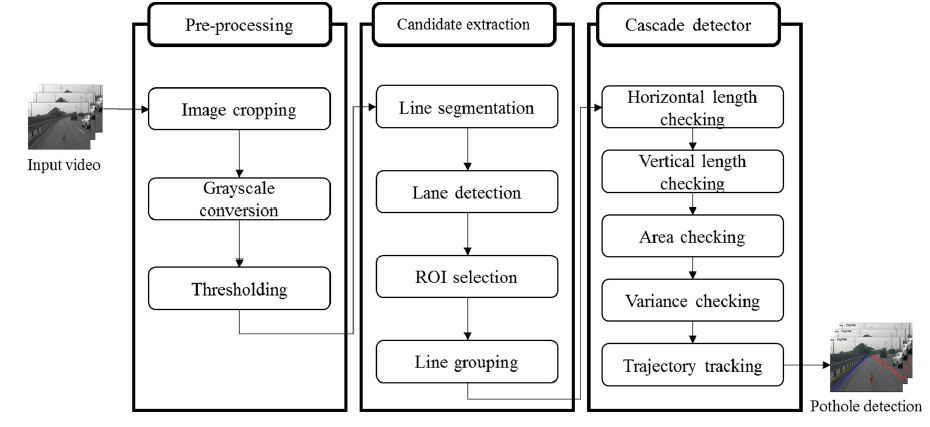
\includegraphics[scale=0.7]{black.png}\centering\caption{Proposed pothole-detection algorithm\cite{Jo}} \label{fig:Proposed pothole-detection algorithm} \end{figure}%

\subsubsection{Results}
In order to determine the accuracy of the proposed method, we manually counted the number of true positives, false positives, and false negatives. We did not count true negatives, because doing so with continuous video data is considerably ambiguous and uncertain.

The Table below shows the performance results for the proposed algorithm according to the number of TPs, FPs, FNs, and its sensitivity and precision. Sensitivity refers to the ratio of correctly detected potholes to actual potholes, and precision refers to the ratio of correctly detected potholes to the total number of detected potholes. The proposed method resulted in an overall sensitivity of 71\%, with 88\% precision\cite{Jo}. 

Thus, the method is more precise than it is sensitive. This means that the algorithm is robust to various kinds of similar objects such as manholes, patches, shade, and moving vehicles. There were fewer FPs than FNs, owing to the diversity of the shape and size of potholes. Moreover, the proposed algorithm wrongly detected potholes that were especially bright or flat.
\begin{table}[H]
\caption{Performance Results \cite{Jo}} % title of Table
\centering % used for centering table
    \begin{tabular}{| l | l |}
	 \hline\hline
    Performance& Values \\ \hline
   TP&22 \\ \hline
    FP&3 \\ \hline
    FN &9 \\ \hline
    Sensitivity(True-Positive rate) &  71\% \\ \hline
   Precision(Positive predicitve value) &  88\% \\ \hline
      		
\end{tabular}
%\label{tab:parameters-sleep-mode} 
\end{table}
We think that the algorithm can be improved by adding more conditions to the cascade detector with only a minimal increase to the algorithm’s complexity. Thus, we confirmed that the proposed pothole-detection system using a black-box camera has can be utilized to collect pothole information. In addition, we expect that our black-box camera with the proposed algorithm can be used successfully as a pothole-alert system, owing to its robustness to similar objects\cite{Jo}.


\section{Detection of Potholes using Image Processing Techniques}
This paper discusses about the detection of potholes using camera installed on light poles of roads. Image processing techniques have been used which informs the officials in a timely manner using email system, thus keeping manual labor to the minimum. For testing its performance, the proposed system has been implemented under a Windows environment using OpenCV library. Simple image processing techniques like canny edge and contour detection with hough transform is used for effective pothole detection\cite{A}.

\subsubsection{Hardware}
The proposed system utilizes a Raspberry Pi, as the main processor for performing the image processing and detecting potholes. A Raspberry Pi is a development board embedded with ARM processor and capable running UNIX based operating system. The model used has an onboard 1GB of RAM, which will make it capable of performing the image processing along with the detection. It also has an interface which supports the raspberry pi to connect to a camera module.
An additional 3G USB modem is utilized as the network interface so that Raspberry Pi is get connected to the internet. This modem attached to Raspberry Pi, therefore it can make the Raspberry Pi is able to transmit any defects or potholes presence on road in real-time\cite{A}.

\subsubsection{Software}
An open-source library of image processing called OpenCV is utilized as the framework for the image processing development. OpenCV is a library which is designed for a computational efficiency for image processing and manipulation.

\subsubsection{Methodology}
\begin{enumerate}[topsep=0pt]

\item Video has been captured using a camera module interfaced with raspberry pi. Frames of the video are extracted and the individual frame is considered as an image which is further processed.

\begin{figure}[H]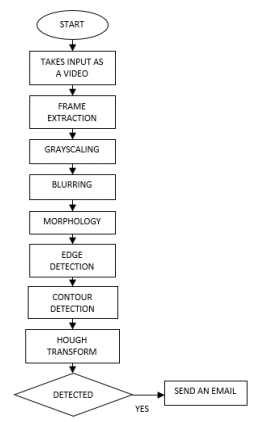
\includegraphics[scale=0.9]{flowchart.png}\centering\caption{Flow chart of image processing\cite{A}} \label{fig:Flow chart of image processing} \end{figure}%

\item The first step after frame extraction was the conversion of the RGB image into grayscale using standard techniques to make processing of image faster.

\item After grayscaling we perform three different blurs on the image. The image is firstly blurred using averaging then with gaussian filter and lastly with median blur so to remove unwanted noise from the image.

\item To achieve more accurate edge detection from a depth image we have modified the process using morphological operations. These operations are generally a collection of nonlinear operations carried out comparatively on the ordering of pixels without affecting their numerical values. The key operators for morphological operations are erosion and dilation\cite{A}.

\item The system then uses contour detection technique. For better accuracy, use binary images. So we have applied threshold and canny edge detection.The contours are a useful tool for shape analysis and object detection and recognition. Thus, it is very useful in pothole detection system.

\end{enumerate}

The system will be installed in a fixed position on the light poles which ensures less handling. Also, this system keeps a track of the negligence and delay. The system makes use of Raspberry Pi, which has a low cost and high compatibility with other interfaces, we also make use of 2D vision-based approach, this makes our system more affordable.  The system also detects potholes in time without damaging the cars for potholes detection. Thus,making the system more feasible and favorable.




\section{Object Detection Algorithms}

Object detection refers to the location of the presence of objects with bounding boxes and types of classes of the located objects in an image.There are mutliple algorithms that deal in object detection like Faster R-CNN\cite{CNN}, YOLO\cite{YOLO} and SSD\cite{SSD}. However for this particular project we used Google's Efficientdet algorithm which consistently achieves much better efficiency than prior algorithms across  several resource constraints.

\subsection{YOLOv3}
YOLO is a single stage detector(SSD). The YOLO algorithm predicta bounding boxes using dimension clusters as anchor boxes. The network predicts 4 coordinates for each bounding box. YOLOv3 predicts the probability or confidence score for each bounding box using logistic regression.This should be one if the bounding box prior overlaps a ground truth object by more than any other bounding box prior\cite{YOLO}.

\begin{figure}[H]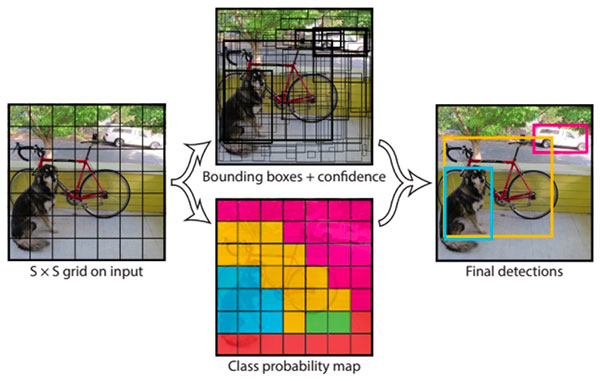
\includegraphics[scale=0.5]{yolo_design.jpg}\centering\caption{Illustration of the YOLO object detector pipeline\cite{YOLO}} \label{fig:Illustration of the YOLO object detector pipeline} \end{figure}%

\subsection{Faster R-CNN}
R-CNN is short for Region--based Convolutional Neural Networks.This algorithm, passes the entire image to ConvNet which generates regions of interest (instead of passing the extracted regions from the image). 
Also, instead of using three different models like the  R-CNN, it uses a single model which extracts features from the regions, classifies them into different classes, and returns the bounding boxes\cite{CNN}.

All these steps are done simultaneously, thus making it execute faster as compared to R-CNN. Fast R-CNN is, however, not fast enough when applied on a large dataset as it also uses selective search for extracting the regions. Selective search identifies a manageable number of bounding box object region candidates/ Region of interest(ROI) and then extracts CNN features from each region independently for classification.

Faster R-CNN fixes the problem of selective search by replacing it with Region Proposal Network (RPN). We first extract feature maps from the input image using ConvNet and then pass those maps through a RPN which returns object proposals. Finally, these maps are classified and the bounding boxes are predicted\cite{CNN}.

\begin{figure}[H]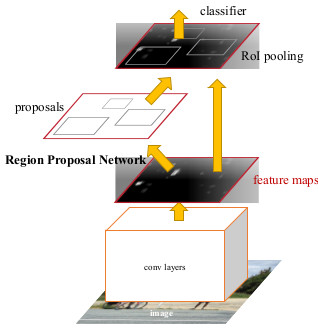
\includegraphics[scale=0.9]{faster-r-cnn-model.jpg}\centering\caption{Architecture of Faster R-CNN\cite{CNN}} \label{fig:Architecture of Faster  RCNN} \end{figure}

\subsubsection{Steps followed in  Faster RCNN to detect objects}

\begin{enumerate}[topsep=0pt]

\item First take an image as an input and pass it through the ConvNet which retuens feature maps.

\item Apply Region Proposal Network(RPN) on these feature maps.

\item Apply ROI pooling layer to bring down all the proposals to the same size

\item Pass these proposals to a fully connected layer in order to classify and predict the bounding boxes for the image.


\end{enumerate}



\subsection{SSD}

SSD is a single-shot detector designed for real time object detection which speeds up the process by eliminating the need for the region proposal network. It applies a few improvements including use of multi-scale features and default boxes. It also predicts the boundary boxes and the classes directly from feature maps in one single pass\cite{SSD}. This algorithm composes of two major parts;

\begin{itemize}[topsep=0pt]

\item Extract feature maps- SSD uses VGG16 to extract feature maps and 

\item Apply convolution filters to detect objects

\end{itemize}

\begin{figure}[h!]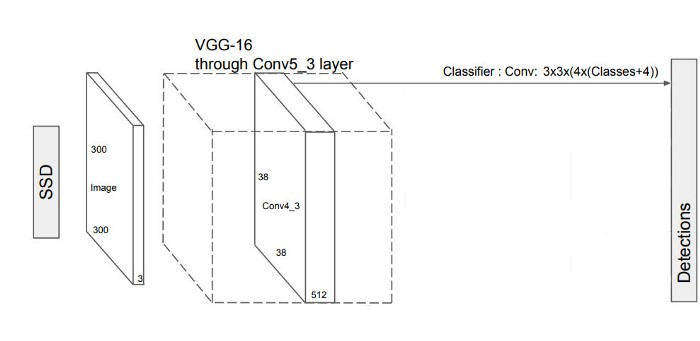
\includegraphics[width=0.8\textwidth]{SSD.jpeg}\caption{SSD Architecture \cite{SSD} }\label{fig:SSD Architecture} \end{figure}%
To improve the accuracy, SSD introduces:

\begin{itemize}[topsep=0pt]

\item Small convolutional filters to predict object classes and offsets to default boundary boxes.

\item Separate filters for default boxes to handle the difference in aspect ratios.

\item Multi-scale feature maps for object detection.
\end{itemize}

SSD can be trained end-to-end for better accuracy, and by removing the delegated region proposal and lowering resolution images, the model can run at real-time speed and still beats the accracy of the state-of-the-art Faster R-CNN\cite{CNN}.

\subsection{EfficientDet}
Efficientdet is a  high efficiency and high accuracy model that works well with small datasets, the image goes through optimization at the different layers. EfficientDet achieves state-of-the-art accuracy while being up to 9x smaller and using significantly less computation compared to prior state-of-the-art detectors\cite{Efficientdet}.


\begin{figure}[h!]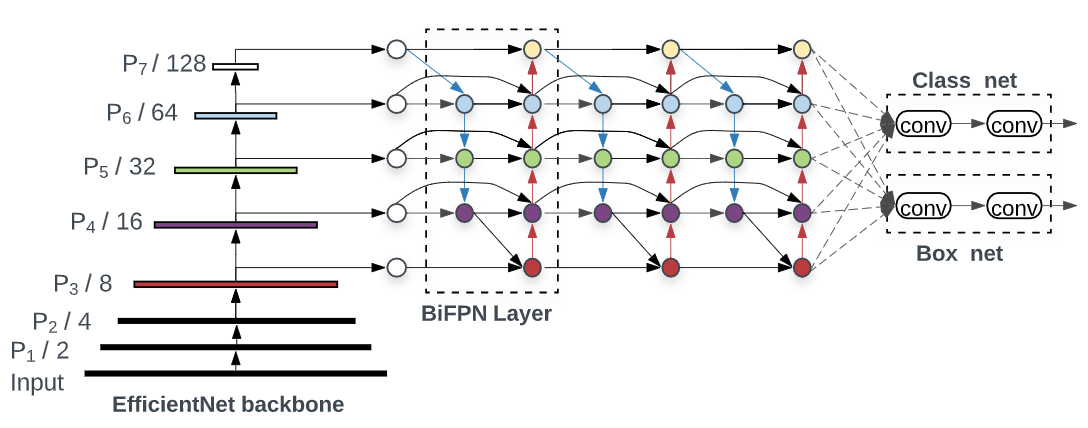
\includegraphics[width=0.9\textwidth]{efficient.png}\caption{Efficientdet Architecture\cite{Efficientdet} }\label{fig:Efficientet} \end{figure}%


 The figure above shows the architecture of the Efficientdet algorithm that consists of three layers  majorly;

\begin{itemize}[topsep=0pt]

\item The backbone which extracts features from a given image. EfficientNet is used as the backbone due to its ability to achieve much better efficiency than other previous detectors like ResNets\cite{Res} or AmoebaNet{Amoeba}.

\item The feature network that takes multiple levelsof features from the backbone as input and outputs a list of fused features that represent salient characteristics of the image. A new bi-directional feature network BiFN which incorporates the multli-level feature fusion that enables information to flow in both the top-down and bottom-up directions while using regular and efficient connections.To improve effieciency, an additional weight is added for each input feature and allow the network to learn the importance of each.
 
\item The class/box network uses the fused features to predict the class and location of each object.This layer involves achieving better accuracy and efficiency trade-offs under different reource constraints.

\end{itemize}

Combining the EfficientNet backbone and the BiFN, a small size EfficientDet--D0 was developed and this was what is used for our model training.
EfficientDet models are 2x-4x faster on GPU, and 5x-11x faster on CPU than other detectors\cite{Efficientdet}.

\subsection{Common Objects in Context (COCO)}
COCO is a large--scale object detection segmentation and captioning datase, tit is widely used in cutting edge image recognition artificial intelligence research.
The COCO dataset is formatted in JSON and is a collection of “info”, “licenses”, “images”, “annotations”, “categories” (in most cases), and “segment info” (in one case)\cite{COCO}.

\subsection{Pascal VOC}
Pascal VOC is an XML file, unlike COCO which has a JSON file. In Pascal VOC we create a file for each of the image in the dataset. In COCO we have one file each, for entire dataset for training, testing and validation\cite{VOC}.

\subsection{Model Performance}
The efficientdet is evaluated on the COCO\cite{COCO} dataset a widely used benchmark dataset for object detection. EfficientDet-D7 achieves a mean average precision(mAP) of 52.2 exceeding the prior state-of-art model by 1.5 points while using 4x fewer parameters and 9.4x less computation. Efficientdet models are also 2x-4x faster on GPU and 5x-11x faster on CPU than other detectors under similar accuracy constraints.


\begin{figure}[H]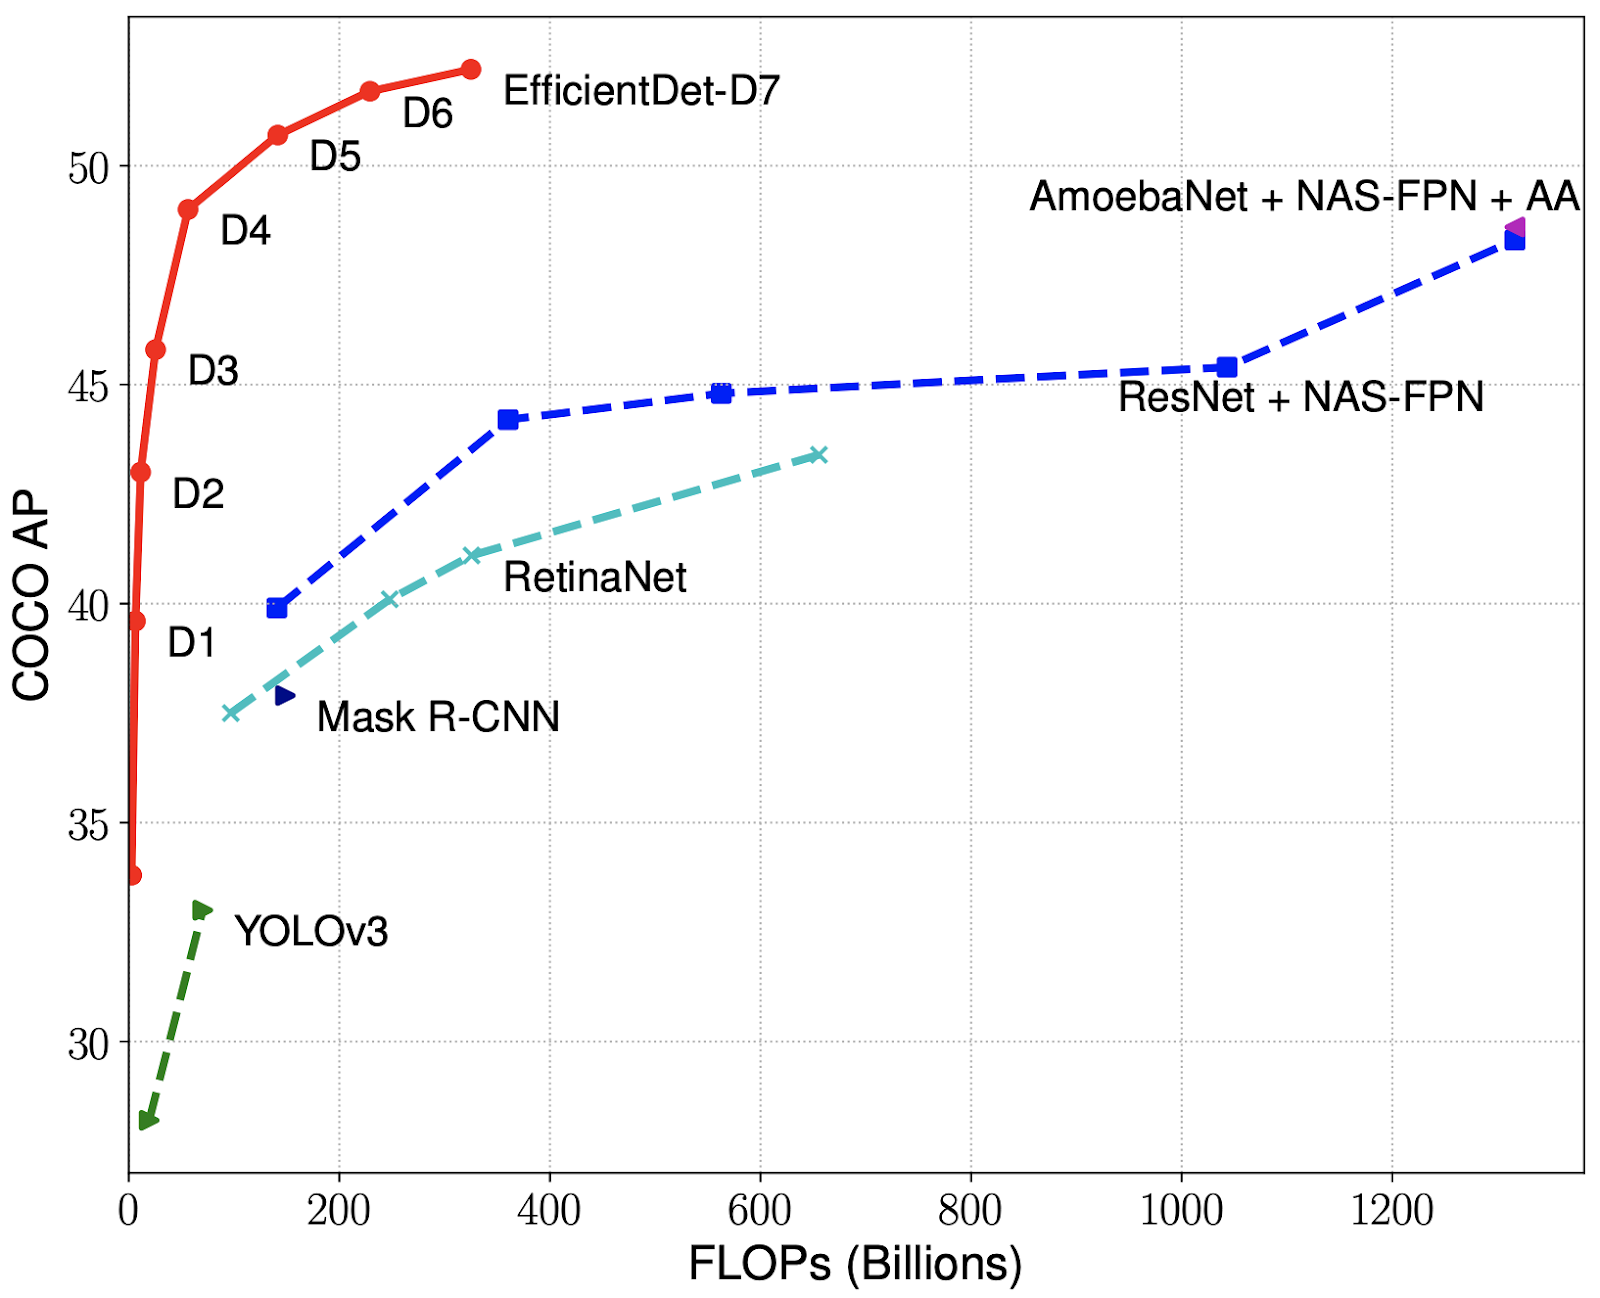
\includegraphics[scale=0.3]{det.png}\centering\caption{Efficientdet Performance with other models \cite{Efficientdet}} \label{fig:Efficientdet performance with other models} \end{figure}%

We have also compared the parameter size and CPU/GPU latency between EfficientDet and previous models. Under similar accuracy constraints, EfficientDet models are 2x-4x faster on GPU, and 5x-11x faster on CPU than other detectors.

While the EfficientDet models are mainly designed for object detection, we also examine their performance on other tasks, such as semantic segmentation. To perform segmentation tasks, we slightly modify EfficientDet-D4 by replacing the detection head and loss function with a segmentation head and loss, while keeping the same scaled backbone and BiFPN. We compare this model with prior state-of-the-art segmentation models for Pascal VOC 2012\cite{VOC}, a widely used dataset for segmentation benchmark.



\begin{table}[H]
\caption{Performance of EfficientDet and DeepLabV3 on PascalVOC 2012\cite{Efficientdet}} % title of Table
\centering % used for centering table
    \begin{tabular}{| l | l | l |}
	 \hline\hline
    Model & mIOU accuracy & FLOPs \\ \hline
    DeepLabV3+(Xception) &  80.2\%&17B \\ \hline
   Our modified EfficientDet &  81.74\%&18B \\ \hline
   
      		
\end{tabular}
%\label{tab:parameters-sleep-mode} 
\end{table}
EfficientDet achieves better quality on Pascal VOC 2012 val than DeepLabV3+ with 9.8x less computation, under the same setting without COCO pre-training.

\subsection{Residual Network (ResNet)}
A residual neural network is an artificical neural network of a kind that builds on constructs known from pyramidal cells in the cerebral cortex\cite{Residual}. 
Mostly in order to solve a complex problem, we stack some additional layers in the Deep Neural Networks which results in improved accuracy and performance.The intuition behind adding more layers is that these layers progressively learn more complex features. But it has been found that there is a maximum threshold for depth with the traditional Convolutional neural network model. This problem has been alleviated with the introduction of ResNets which are made up of Residual Blocks.

\begin{figure}[H]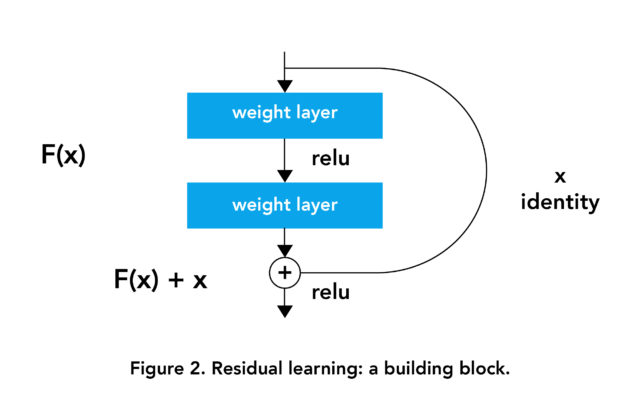
\includegraphics[scale=2]{resnet.jpg}\centering\caption{Residual Block \cite{Res}} \label{fig:Residual Block} \end{figure}%

With the blocks, there is a direct connection which skips some layers in between. This connection is called skip connection and is the core of residual blocks.
The skip connections in ResNet solve the problem of vanishing gradient in deep neural networks by allowing this alternate shortcut path for the gradient to flow through. The other way that these connections help is by allowing the model to learn the identity functions which ensures that the higher layer will perform at least as good as the lower layer, and not worse\cite{Res}.

\subsection{AmoebaNet}
AmoebaNet is a convolutional neural network found through regularized evolution architecture search. The search space is NASNet, which specifies a space of image classifiers with a fixed outer structure\cite{Amoeba}. 

Inorder to solve the problem that the network architecture parameters cannot be updated by the gradient propagation of the verficiation set accuracy,some scholars have proposed the idea of reinforcement learning to optimize the controller RCNN. The evolutionary algorithm also doesn't need to calculate the loss function or gradient propagation of the objective function and only requires some simple and easy-to-operate encoding processing to optimize the objective function\cite{Am}.




%\section{Summary}
% End your chapter with a short summary.






























\chapter{Methodolgy}

\section{Introduction}

This chapter includes the techniques, tools and procedures that were used inorder to design the pothole detection system.These procedures were divided into four stages that are explained in detail below. These include  Image Collection, Image Pre-Processing , Model Training and Evaluation.

\begin{figure}[h!]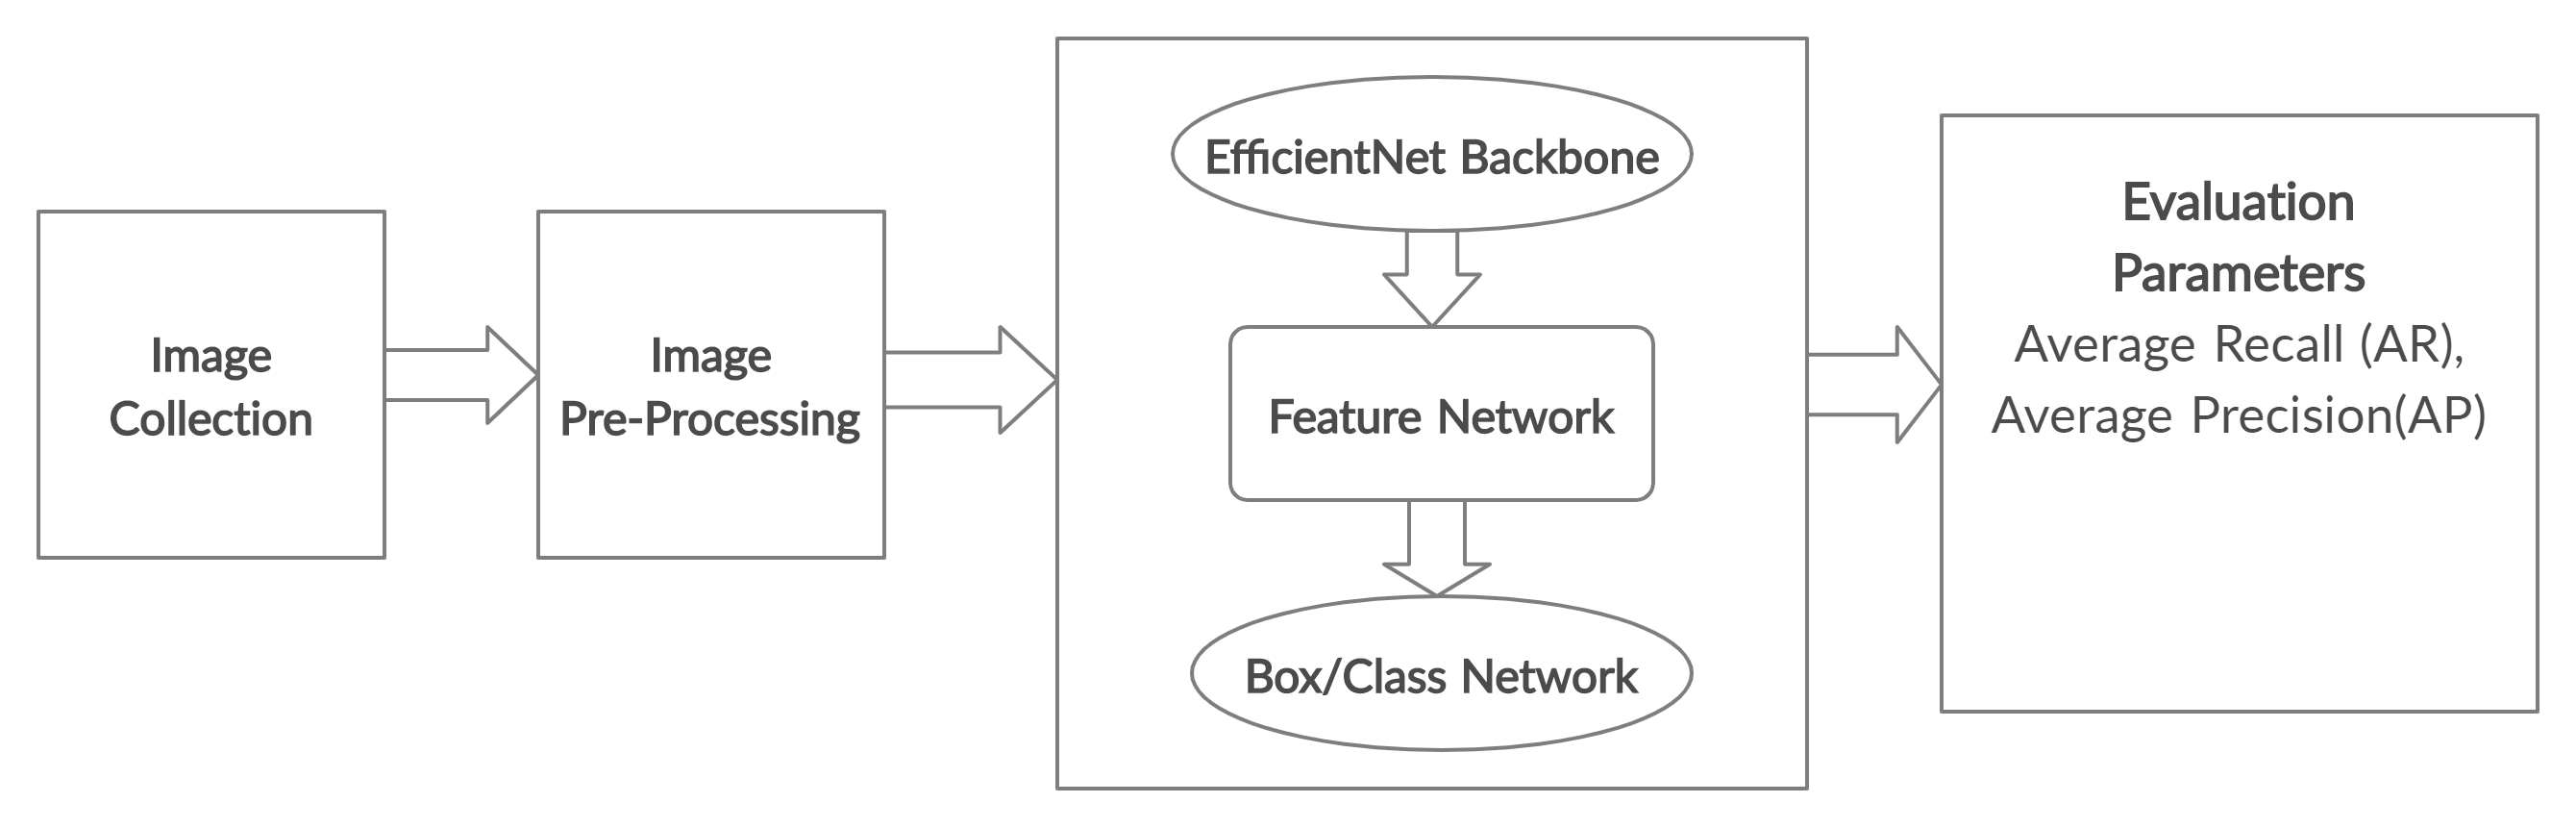
\includegraphics[width=0.9\textwidth]{Methodology (2).png}\caption{Methodolgy} \label{fig:methodology} \end{figure}%

\section{Image Collection}

Images were taken from  few selected roads that presented with quite a number of potholes by use of a mobile phone.

\begin{itemize}[topsep=0pt]
 
\item A smart mobile phone with a camera was mounted onto a windscreen phone holder and the images taken in form of videos.A Techno Camon 11 32GB storage and a Samsung Galaxy S8 64GB storage were the smart phones used for image collection.

\begin{figure}[H]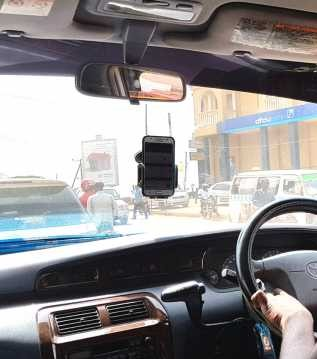
\includegraphics[scale=0.6]{phone.jpg}\centering\caption{Phone on a windscreen} \label{fig:Phone on windscreen} \end{figure}%

\item  Using VLC Media Player the videos taken were sliced into multiple images.

\item  The images were sorted to retain those that displayed potholes and eliminate the duplicates.
\end{itemize}

\section{Image Pre-Processing}

Image pre-processing involves preparing the dataset for the training stage.It involves resizing the images, labelling the images and  extracting useful information into different formats required for model training.
\begin{itemize}[topsep=0pt]

\item The images were resized by using Smart Resize and also renamed.

\item The images were then uploaded to Labelbox which is also where all our pothole images are to be stored.% Lablebox is an online application that has labelling tools that enable humans to create data ready to be consumed by the training algorithm.

\item  With Labelbox, the images were labelled by drawing bounding boxes around those areas in the image with pothole.

\item A json file was generated from labelbox that contained information required for the training stage.

\item For the object detection specifications, we had one class which is potholes as we were not considering those images without potholes.

\item The dataset was split into the train, test and validation set of images.The training dataset is the images that we used in the training of the model,the validation dataset provides an unbiased evaluation of the model fit on the training dataset while tuning model hyperparameters, the test dataset is used to provide an unbiased evaluation of a final trained model.

\item For each of the datasets a COCO json file was generated as it is the required format for training our model.%COCO is a large-scale object detection,segmentation and captioning dataset.-literature review

\item For the training of the model tf records are used, these store data as a sequence of binary strings and take up less space on disk.The records were generated from the dataset images and their coresponding COCO json file generated.

\end{itemize}

\section{Model Training}

For the model Training Google colab notebook was used and Google Efficientdet algorithm was used due to its  high accuracy and high efficiency characteristics that can be used for small size datasets.

\begin{itemize}[topsep=0pt]

\item For the training of the model efficientDet--d0 object detection model was used because of the input image size, its small size dataset characteristic which is specific to this dataset and also it goes upto three classes, in this case we deal with one class\cite{det}.

\item For the training, tf records are required,the eval batch size which is the amount of dataset that is fed into the model during the evaluation process of training, the number of epochs which is the number of complete passes through the training dataset.

\item  The training environment was set-up in Google colab by installing efficientDet-d0, COCO dataset API and Tensorflow environment and the training of the model initiated.

\item The trained model was saved onto google drive so it can be used on the test images, to test the trained model accuracy.

\end{itemize}

\section{Hardware used for Training the model}

\subsection{Google Colab}
Google Colaboratory is a free online cloud-based jupyter notebook environment that allows you to train your macihine learning model, data analysis and education purposes.It also allows colloboration and sharing work among team members. Google Colab provides you with free GPUs,CPUs and TPUs and memory for your training session.
Google Colab was used in this project for the model training due to its nature, we could access free runtime for training our model at very high speeds\cite{Colab}.

A Graphics Processing Unit (GPU) is a microprocessing chip designed to handle Graphics in computing environments. GPUs can have hundreds and even thousands of more cores than a Central Processing Unit (CPU).
 GPUs are optimized for training artificial intelligence and deep learning models as they can process multiple computations simultaneously\cite{GPU}.

\subsection {Labelbox}
Labelbox is a collaborative training data platform that enables one create labeled data by drawing bounding boxes around the specific objects in the image and also is a database for your labeled images. Labelbox also enables one to generate a jsonfile that includes all the image information like each bounding box coordinates for every object labelled in an image\cite{labelbox}.

\subsection {Smartresize}
Smart Resize is an online tool that enables one to resize their images in bulk to any dimension of their choice. All it requires is to have the data stored on your local machine or cloud and then upload it to smart resize and fill in the dimension you require, and everything will be worked on\cite{Smartresize}.

\section{Frameworks and Libraries used in Training}
\subsection{Tensorflow}
TensorFlow is an open source library for numerical computation and large-scale machine learning. TensorFlow bundles together a slew of machine learning and deep learning (aka neural networking) models and algorithms and makes them useful. It uses Python to provide a convenient front-end API for building applications with the framework, while executing those applications in high-performance C++.

TensorFlow can train and run deep neural networks for handwritten digit classification, image recognition, word embeddings, recurrent neural networks, sequence-to-sequence models for machine translation, natural language processing.

TensorFlow allows developers to create dataflow graphs—structures that describe how data moves through a graph, or a series of processing nodes. 

TensorFlow provides for machine learning development is abstraction. Instead of dealing with the nitty-gritty details of implementing algorithms, or figuring out proper ways to hitch the output of one function to the input of another, the developer can focus on the overall logic of the application. TensorFlow takes care of the details behind the scenes\cite{Tensor}



\subsection{Pandas}
Pandas is a Python package that provides fast, flexible, and expressive data structures designed to make working with structured (tabular, multidimensional, potentially heterogeneous) and time series data both easy and intuitive. It aims to be the fundamental high-level building block for doing practical, real world data analysis in Python\cite{Pandas}.
Pandas take on data like CSV files  and create a python object with rows and coulmns called dataframes.

\subsection{Numerical Python(NumPy)}
NumPy is is a linear algebra library in Python. It is a very important library on which almost every data science or machine learning Python packages such as SciPy (Scientific Python) and Scikit-learn, etc depends on to a reasonable extent.

NumPy is very useful for performing mathematical and logical operations on Arrays. It provides an abundance of useful features for operations on n-arrays and matrices in Python\cite{Num}.

\subsection{Matplotlib}
Matplotlib is an open-source plotting library in Python introduced in the year 2003. It is a very comprehensive library and designed in such a way that most of the functions for plotting in MATLAB can be used in Python.
It consists of several plots like the Line Plot, Bar Plot, Scatter Plot, Histogram e.t.c through which we can visualise various types of data.
In this project, we used matplot to visualize our labelled images and verfiy if the bounding boxes were in the right areas\cite{Mat}.

\subsection{Hardware Specifications Used}
For Training the model, the Google Colab jupyter notebook was set to the specifications below:

\begin{itemize}[topsep=0pt]

\item Python 3 Google Compute Engine backend (GPU)

\item RAM- 12.72 GB 

\item Disk -64.40 GB

\item Tensorflow version- tensorflow.compact.v1

\end{itemize}



% Add sections and (sub)subsections as appropriate
\section{Model Evaluation}
The model performance is evaluated on several set parameters.

\subsection{Evaluation Paramters}
Evaluation Parameters or Metrics explain the performance of a model and enable you get feedback that can improve the performance of the model.


\subsection {Average Precision (AP) }
Is the measure of accuracy of object detection.
\begin{itemize}[topsep=0pt]

\item AP =$\dfrac{True Positive}{True Positive + False Positive}$
\end{itemize}


\subsection {Average Recall (AR)}
This is the measure of how good you find the positives.

\begin{itemize}[topsep=0pt]
\item AR =$\dfrac{True Positive}{True Positive + False Negative}$
\end{itemize}


\subsection {Intersection over Union (IoU)}
Intersection Over Union is an evaluation metric used to measure the accuracy of an object detectoron a particular dataset. It is a good number from 0 to 1 that specifies the amount of overlap between the predicted and ground truth bounding box\cite{IoU}.

\begin{itemize}[topsep=0pt]
\item an IoU of 0 means that there is no overlap between the boxes.

\item an IoU of 1 means that the union of boxes is the same as their overlap indicating that they are completely overlapping.
\end{itemize}


\begin{figure}[H]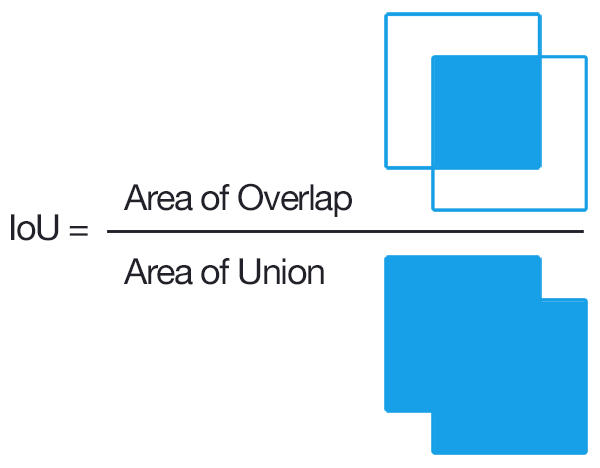
\includegraphics[scale=0.5]{IoU.png}\centering\caption{Intersection over Union}\cite{IoU} \label{fig:Intersection over Union} \end{figure}%





% Add other chapters and their (sub)(sub)sections as appropriate







\chapter{ Results}
This chapter contains results from the different stages in the methodolgy carried out in this project.
\begin{itemize}[topsep=0pt]

\item A total of 836 dataset of  pothole images were collected from Bombo road, Acacia Avenue, Sir Apollo Kaggawa, Lugogo bypass, Mary Stuart- Lumumba Hall road, Entebbe- Kampala road.

\begin{figure}[H]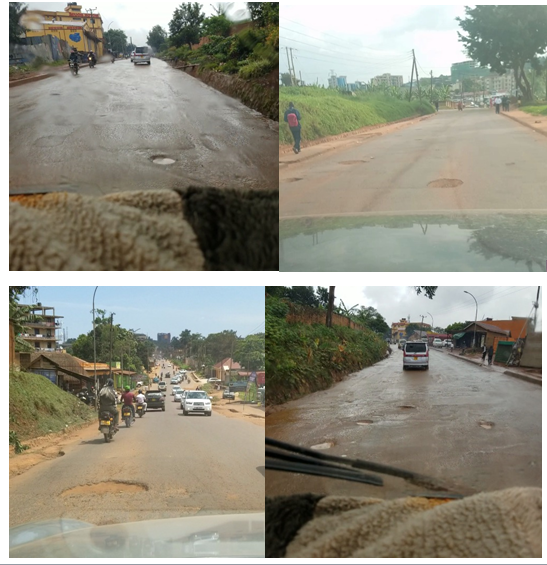
\includegraphics[scale=0.9]{pothole.png}\centering\caption{Samples of images collected} \label{fig:Sample of images collected} \end{figure}%

\item With the use of Labelbox online tool , images were labelled by drawing boounding boxes around the areas with potholes.

\begin{figure}[H]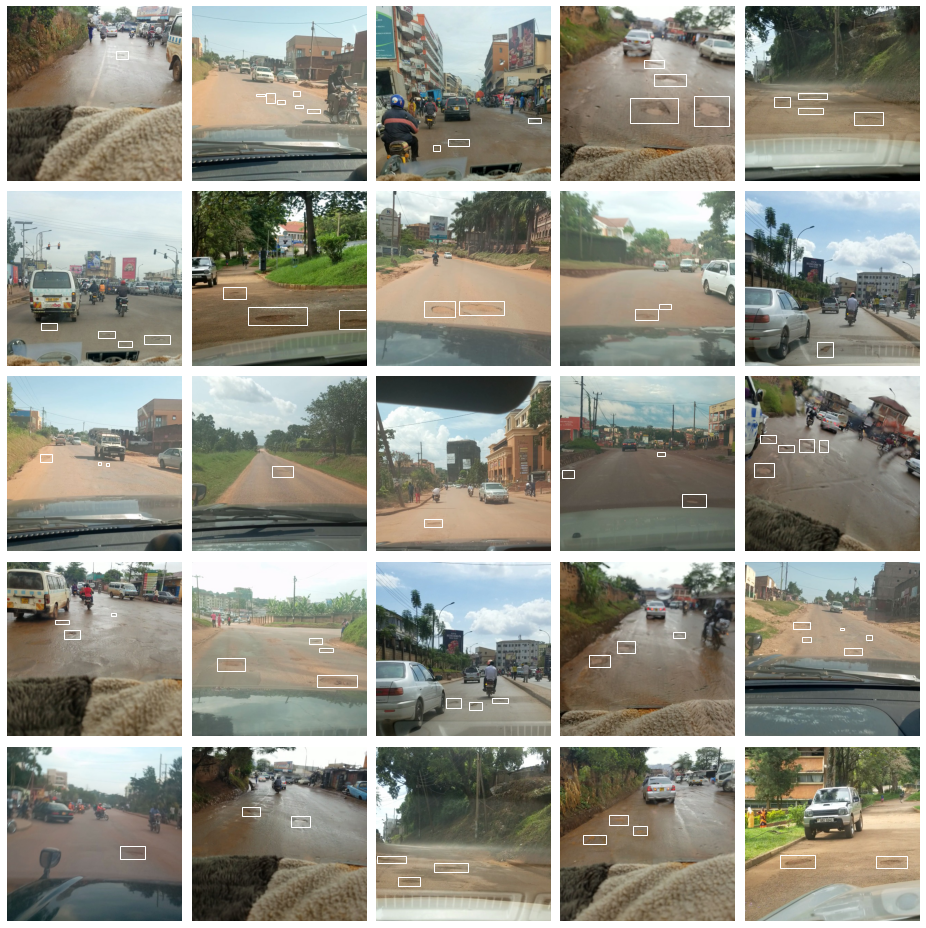
\includegraphics[scale=0.4]{label2.png}\centering\caption{Labelled images} \label{fig:Labelled images} \end{figure}%

\item The dataset was split into the training set -587 images, test set -84 images and validation set -167 images.

\item For the training phase, the eval batch size was set to 20, 20 batch of images were fed into the model per cycle during the evaluation process of training while the number of epochs was set to 50 meaning 50 complete passes through the training dataset.

\item The training phase took 2 hours and the trained model saved to google drive so that it can be used on the test dataset.

\end{itemize}


\begin{table}[H]
\section{Parameter Table}
This table contains results of the AP and AR at different IoU percentages to showing the different accuracy at this percentages.
\caption{Parameter Results} % title of Table
\centering % used for centering table
    \begin{tabular}{| l | l |}
	 \hline\hline
    Parameters & Values \\ \hline
    Average Precision (AP) @ IoU =0.50 &  0.720 \\ \hline
    Average Precision (AP) @ IoU =0.75 &  0.300 \\ \hline
    Average Precision (AP) @ IoU =0.50:0.95 &  0.196 \\ \hline
    Average Recall (AR) @ IoU =0.50:0.95 &  0.189 \\ \hline
      		
\end{tabular}
%\label{tab:parameters-sleep-mode} 
\end{table}

% Usually, start with a table of parameters similar to the one below, if this applies to your project.
\section{Graphs}
Tensorboard is a visualization toolkit that enables one to track and visualize model graphs of loss, accuracy and other metrics. The tensorboard was activated during the training of the model to observe how the training was going in form of graphs. The graphs below are what was generated from tensorboard.

The graph below indicates how the accuracy of the model increases as the number of training steps increase during training of the nodel. An average precision of 0.52515274 was obtained at AP50.
\begin{figure}[H]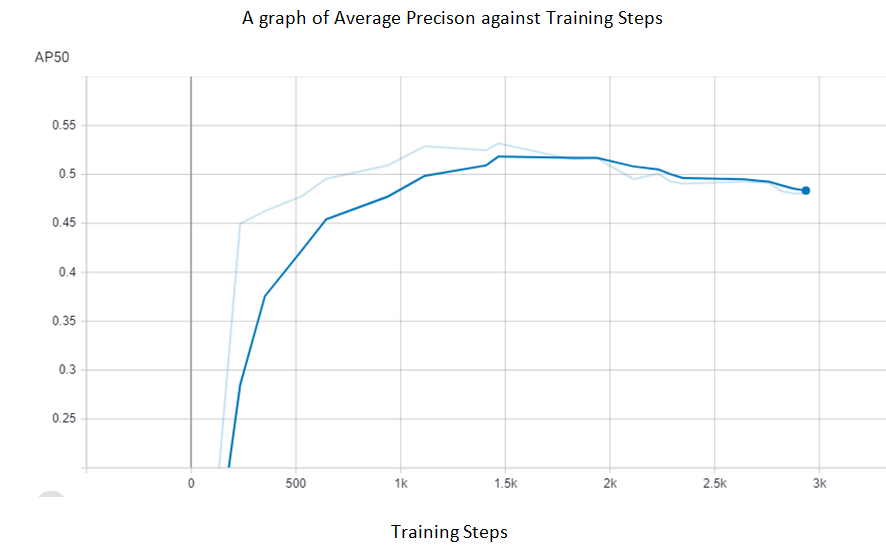
\includegraphics[scale=0.5]{AP50.png}\centering\caption{A graph of AP50 against Training Steps} \label{fig:AP50 against Training Steps} \end{figure}%

The graph below indicates how good positive bounding boxes have been found given 100 detections per image against the training steps.
\begin{figure}[H]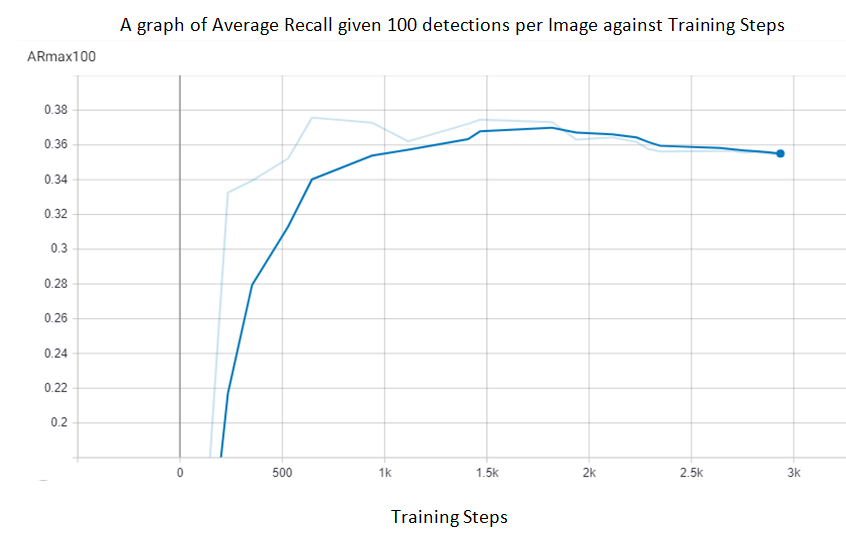
\includegraphics[scale=0.6]{ARmax.png}\centering\caption{A graph of ARmax against Training Steps} \label{fig:ARmax against Training Steps} \end{figure}%

\section{Images}
Below are images taken to test if our model can detect potholes accurately. In the test images, an accuracy percentage is placed on the pothole detection.
\begin{figure}[H]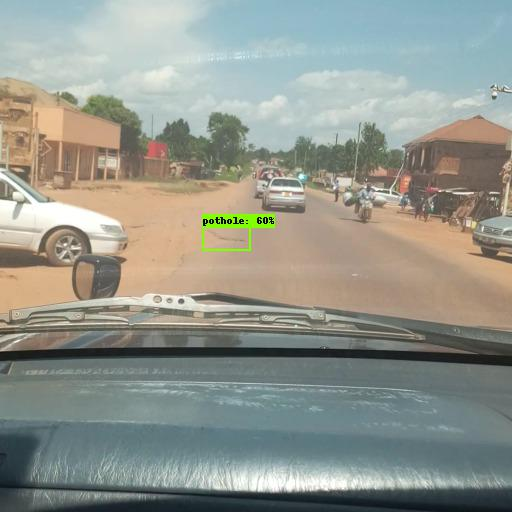
\includegraphics[scale=0.6]{1.jpg}\centering\caption{Test images and degree of accuracy of the detection} \label{fig:Test Images} \end{figure}%
\begin{figure}[H]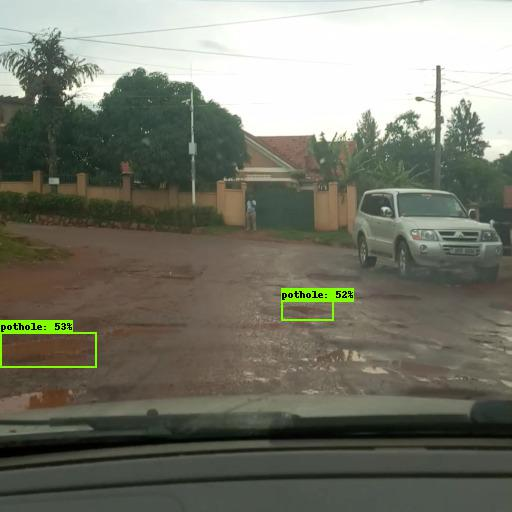
\includegraphics[scale=0.6]{2.jpg}\centering\caption{Test images and degree of accuracy of detection} \label{fig:Test Images} \end{figure}%
\begin{figure}[H]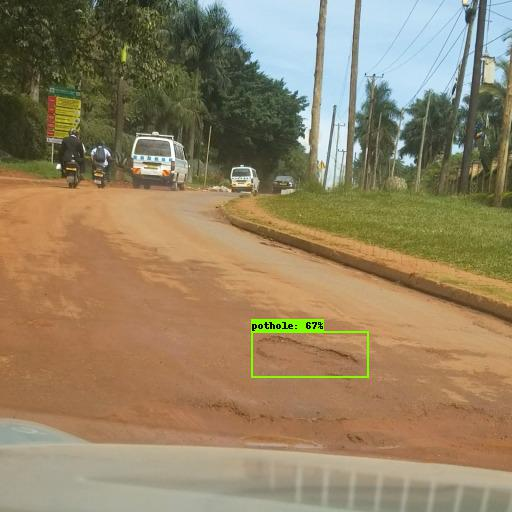
\includegraphics[scale=0.6]{3.jpg}\centering\caption{Test images and degree of accuracy of detection} \label{fig:Test Images} \end{figure}%
\begin{figure}[H]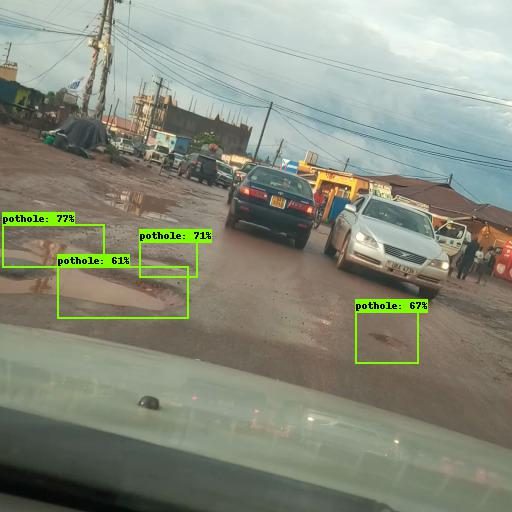
\includegraphics[scale=0.6]{5.jpg}\centering\caption{Test images and degree of accuracy of detection} \label{fig:Test Images} \end{figure}%
\begin{figure}[H]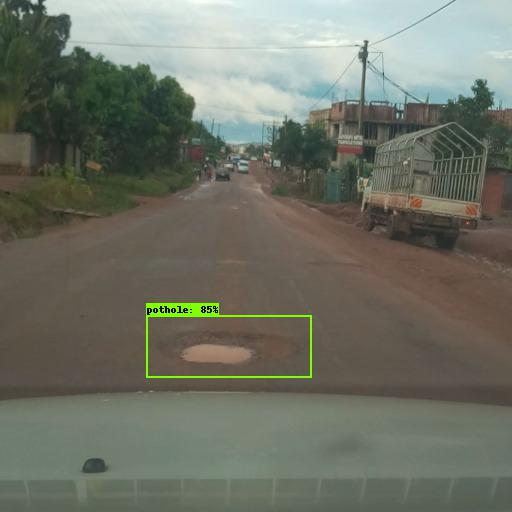
\includegraphics[scale=0.6]{6.jpg}\centering\caption{Test images and degree of accuracy of detection} \label{fig:Test Images} \end{figure}%
% End with a conclusion chapter
\chapter{Conclusions and Future Works}
%\label{chap:conclusion}

\section{Conclusions}

%Conclude here
In this project, we developed a dataset of 836 pothole images from Acacia Avenue, Bombo road, Sir Apollo Kaggawa, Lugogo Bypass, Jinja road, Entebbe-Kampala Road, Yusuf Lule, Mary Stuart-Lumumba Hall road and Gayaza Road.
We trained and evaluated a machine learning model that can detect potholes using the collected pothole images. Based on the results, we attained a mean Average Precision of 0.52515274.We believe that this pothole detection model will be a useful resource to the authorities concerned with road maintenance and repair.

\section{Ideas for Future Work}
\begin{itemize}[topsep=0pt]

\item Collect more images of potholes from other roads around the city and also outside the city and use these on our model so it can become better at detecting potholes.

\item Train the pothole image dataset on other object detection algorithms like YOLOv5, Mask R-CNN and SSD and be able to compare their performances with ourtrained model.

\end{itemize}
% You can also add a section on challenges and recommendations if you wish













%\bibliographystyle{alpha}

\bibliographystyle{IEEEtran}


\begin{thebibliography}{1}
\bibitem{Roads}
“Maintenance of National Roads: What are the key challenges?,” 2019 [Online]. Available: https://www.finance.go.ug/sites/default/files/Publications/BMAU Policy Brief 21-19-Maintenance of National Roads- What are the key challenges.pdf. [Accessed: 21-Dec-2020]. 

\bibitem{Road--Fund}
http://www.oag.go.ug/wp-content/uploads/2016/07/Report-Efficiency-of-uganda-Road--Fund.pdf. ''[Online]. [Accessed 10-September-2019]

\bibitem{AI}
“Artificial Intelligence (AI) Definition.” [Online]. Available: https://www.investopedia.com/terms/a/artificial-intelligence-ai.asp. [Accessed: 19-Dec-2020].


\bibitem{Machine--Learning}
“What is Machine Learning? A definition - Expert System | Expert.ai.” [Online]. Available: https://www.expert.ai/blog/machine-learning-definition/. [Accessed: 17-Dec-2020].

\bibitem{Difference}
“AI, ML and DL: What’s the difference?| by Roberta Nicora | Dative\_io | Medium.” [Online]. Available: https://medium.com/dative-io/ai-ml-and-dl-whats-the-difference-86a8af387150. [Accessed: 19-Dec-2020].


\bibitem{Supervised}
“What is machine learning? Everything you need to know | ZDNet.” [Online]. Available: https://www.zdnet.com/article/what-is-machine-learning-everything-you-need-to-know/. [Accessed: 17-Dec-2020].

\bibitem{Super}
“Supervised and Unsupervised Machine Learning Algorithms.” [Online]. Available: https://machinelearningmastery.com/supervised-and-unsupervised-machine-learning-algorithms/. [Accessed: 17-Dec-2020].

\bibitem{Unsupervised}
“Unsupervised Machine Learning: What is, Algorithms, Example.” [Online]. Available: https://www.guru99.com/unsupervised-machine-learning.html. [Accessed: 17-Dec-2020].

\bibitem{Vision}
“Computer vision - Wikipedia.” [Online]. Available: https://en.wikipedia.org/wiki/Computer\_vision. [Accessed: 19-Dec-2020].

\bibitem{Deep-Learning}
“Deep learning vs machine learning.” [Online]. Available: https://www.zendesk.com/blog/machine-learning-and-deep-learning//. [Accessed: 17-Dec-2020].

\bibitem{Y.J.Cha}
Y. J. Cha, W. Choi, and O. Buyukozturk, “Deep Learning-Based Crack Damage Detection Using Convolutional Neural Networks,” Comput. Civ. Infrastruct. Eng., vol. 32, no. 5, pp. 361–378, 2017.

\bibitem{Raghav}
“Understanding of Convolutional Neural Network (CNN) — Deep Learning | by Prabhu | Medium.” [Online]. Available: https://medium.com/RaghavPrabhu/understanding-of-convolutional-neural-network-cnn-deep-learning-99760835f148. [Accessed: 17-Dec-2020].

\bibitem{Neural}
“(PDF) Road Damage Detection Using Deep Neural Networks with Images Captured Through a Smartphone.” [Online]. Available: https://www.researchgate.net/publication  322787719\_Road\_Damage\_Detection\_Using\_Deep\_Neural\_Networks\_with\_Images\_Captured\_Through\_a\_Smartphone. [Accessed: 17-Dec-2020].

\bibitem{Jo}
Y. Jo and S. Ryu, “Pothole detection system using a black-box camera,” Sensors (Switzerland), vol. 15, no. 11, pp. 29316–29331, 2015.

\bibitem{A}
A. Bhat, P. Narkar, D. Shetty, and D. Vyas, “Detection of Potholes using Image Processing Techniques,” 2018.

\bibitem{YOLO}
https://www.pyimagesearch.com/2018/11/12/yolo-object-detection-with-opencv/

\bibitem{CNN}
“Faster RCNN Python | Faster R-CNN For Object Detection.” [Online]. Available: https://www.analyticsvidhya.com/blog/2018/11/implementation-faster-r-cnn-python-object-detection/?utm\_source=blog\&utm\_medium=a-step-by-step-introduction-to-the-basic-object-detection-algorithms-part-1. [Accessed: 20-Dec-2020].

\bibitem{SSD}
“SSD object detection: Single Shot MultiBox Detector for real-time processing | by Jonathan Hui | Medium.” [Online]. Available: https://jonathan-hui.medium.com/ssd-object-detection-single-shot-multibox-detector-for-real-time-processing-9bd8deac0e06. [Accessed: 19-Dec-2020].

\bibitem{Efficientdet}
https://ai.googleblog.com/2020/04/efficientdet-towards-scalable-and.html

\bibitem{COCO}
“Create COCO Annotations From Scratch — Immersive Limit.” [Online]. Available: https://www.immersivelimit.com/tutorials/create-coco-annotations-from-scratch/[Accessed: 22-Dec-2020].

\bibitem{VOC}
“COCO and Pascal VOC data format for Object detection | by Renu Khandelwal | Towards Data Science.” [Online]. Available: https://towardsdatascience.com/coco-data-format-for-object-detection-a4c5eaf518c5. [Accessed: 20-Dec-2020].

\bibitem{Residual}
“Residual neural network - Wikipedia.” [Online]. Available: https://en.wikipedia.org/wiki/Residual\_neural\_network. [Accessed: 19-Dec-2020].

\bibitem{Res}
“What is Resnet or Residual Network | How Resnet Helps?” [Online]. Available: https://www.mygreatlearning.com/blog/resnet/. [Accessed: 19-Dec-2020].

\bibitem{Amoeba}
“AmoebaNet Explained | Papers With Code.” [Online]. Available: https://paperswithcode.com/method/amoebanet. [Accessed: 19-Dec-2020].

\bibitem{Am}
“AmoebaNet paper and algorithm analysis - Programmer Sought.” [Online]. Available: https://www.programmersought.com/article/34154613408/. [Accessed: 19-Dec-2020].

\bibitem{det}
“Google AI Blog: EfficientDet: Towards Scalable and Efficient Object Detection.” [Online]. Available: https://ai.googleblog.com/2020/04/efficientdet-towards-scalable-and.html. [Accessed: 17-Dec-2020].


\bibitem{Colab}
“How to Use Google Colab for Deep Learning and Machine Learning.” [Online]. Available: https://www.analyticsvidhya.com/blog/2020/03/google-colab-machine-learning-deep-learning/. [Accessed: 17-Dec-2020].

\bibitem{GPU}
“The Complete Guide to Deep Learning with GPUs - MissingLink.ai.” [Online]. Available: https://missinglink.ai/guides/computer-vision/complete-guide-deep-learning-gpus/. [Accessed: 21-Dec-2020].

\bibitem{labelbox}
“Labelbox - Crunchbase Company Profile \& Funding.” [Online]. Available: https://www.crunchbase.com/organization/labelbox. [Accessed: 17-Dec-2020].

\bibitem{Smartresize}
“Smart Resize - Fastest \& smartest bulk online image resizer.” [Online]. Available: https://www.smartresize.com/. [Accessed: 22-Dec-2020].

\bibitem{Tensor}
“What is TensorFlow? The machine learning library explained | InfoWorld.” [Online]. Available: https://www.infoworld.com/article/3278008/what-is-tensorflow-the-machine-learning-library-explained.html. [Accessed: 21-Dec-2020].

\bibitem{Pandas}
“pandas . PyPI.” [Online]. Available: https://pypi.org/project/pandas/. [Accessed: 21-Dec-2020].

\bibitem{Num}
“Let’s talk about NumPy — for Data Science Beginners | by Ehi Aigiomawu | Towards Data Science.” [Online]. Available: https://towardsdatascience.com/lets-talk-about-numpy-for-datascience-beginners-b8088722309f. [Accessed: 21-Dec-2020].

\bibitem{Mat}
“Matplotlib for Machine Learning. Matplotlib is one of the most popular by Paritosh Mahto | MLpoint | Medium.” [Online]. Available: https://medium.com/mlpoint/matplotlib-for-machine-learning-6b5fcd4fbbc7. [Accessed: 21-Dec-2020].

\bibitem{IoU}
“IoU a better detection evaluation metric | by Eric Hofesmann | Towards Data Science.” [Online]. Available: https://towardsdatascience.com/iou-a-better-detection-evaluation-metric-45a511185be1. [Accessed: 22-Dec-2020].

%\bibitem{cisco}
%Cisco, "Cisco Visual Networking Index: Forecast and Trends, 2017–2022 White Paper \emph{Cisco Systems.Inc}, Document ID:1551296909190103, Updated February 27, 2019.

%\bibitem{bisect} R. L. Burden and J. D. Faires, Numerical Analysis: Bisection Method, 9th Ed., Brooks/Cole, Cengage Learning, 20 Channel Center Street, Boston, MA 02210, USA, 2011.

\end{thebibliography}


%% the bibliography style determines the format  in which both citations and references are printed,
%% other possible values are plain and abbrv
%%
%% If you want more control of the format of your citations you might want to take a look at
%% natbib.sty, which should be part of any standard LaTeX installation
%%
%% University regulations simply require that your citation style be consistent, so see what style
%% your supervisor recommends.

% Appendices start here



\appendix

\chapter{Appendix}
\section{Code for creating COCO json file and CSV files}

\begin{lstlisting}

def get_json(dir):
    """Get *.json files in dir."""
    jsons = []
    for file in os.listdir(dir):
        if file.endswith(".json"):
            jsons.append(os.path.join(dir, file))
    return jsons

def process_labelbox_json(jsons):
    """
        Parse Labelbox labels JSON.
    """
    df = pd.DataFrame(columns=['file_name',
                                'xmin',
                                'ymin',
                                'width',
                                'height'])
    
    # Extract
    for file in jsons:
        f = open(file, 'r')
        data = json.load(f)
        f.close()
        
        for item in tqdm(data, desc="Processing data: "):
            # print ('Working')
            item_label = item['Label']

            # check if the item['Label'] is empty. If empty, continue to the next item.
            if bool(item_label)==False:
                continue

            # check if the item['Label']['objects'] is empty, if so, proceed to the next item.
            elif bool(item_label['objects']==False):
                continue

            # All  is well, execute the loop below for all the bounding boxes.
            #Image file_name
            file_name = item['External ID']

            #Extract the bounding boxes
            for bounding_box in item_label['objects']:
                # print(dictionary['bbox'])

                # class_name = bounding_box['title'].replace(" ", "")

                ymin = bounding_box['bbox']['top']
                xmin = bounding_box['bbox']['left']

                height = bounding_box['bbox']['height']
                width = bounding_box['bbox']['width']

                df = df.append({"file_name": file_name,
                                "xmin": xmin,
                                "ymin": ymin,
                                "width": width,
                                "height": height},
                                ignore_index=True)
            
    return df
    

   

def make_dirs(dirs):
    """Make directories that don't exist."""
    for dir in dirs:
        if not os.path.isdir(dir):
            os.mkdir(dir)
            

def split_indices(x, train=0.8, test=0.0, validate=0.2, shuffle=True):  
    # split training data
    n = len(x)
    v = np.arange(n)
    if shuffle:
        np.random.shuffle(v)

    i = round(n * train)  # train
    j = round(n * test) + i  # test
    k = round(n * validate) + j  # validate
    return v[:i], v[i:j], v[j:k]  # return indices

def split_files(file_names,train=0.8, test=0.2, validate=0.0):  # split training data
    file_name = list(filter(lambda x: len(x) > 0, file_names))
    file_name = sorted(file_name)
    i, j, k = split_indices(file_names, train=train, test=test, validate=validate)
    train = []
    test = []
    val = []
    datasets = {'train': i, 'test': j, 'val': k}
    for key, item in datasets.items():
        if item.any():
            for ix in item:
                if key == 'train':
                  train.append(file_names[ix])
                if key == 'test':
                    test.append(file_names[ix])
                if key == 'val':
                    val.append(file_names[ix])

    return train, test, val
# create coco file
def make_coco_file(labels, categories, filenames):
    """Creates a COCO format data structure."""

    classes = sorted(categories)
    category_list = []

    # COCO ANNOTATION FORMAT
    for i, category in enumerate(classes):
        foo = {}
        foo["supercategory"] = "None"
        foo["id"] = i + 1 # COCO is one-indexed
        foo["name"] = category
        category_list.append(foo)

    # COCO VARIABLE
    COCO_DATA = {}
    COCO_DATA["type"] = "instances"
    COCO_DATA["images"] = []
    COCO_DATA["annotations"] = []
    COCO_DATA["categories"] = category_list

    image_id = 0 # Image id
    annotation_id = 0 # Annotation id

    label = "pothole" # Different implementation for more than one label

    # Iterate through the filenames
    for file_name in tqdm(filenames, desc="Creating COCO: "):

        # Add to COCO images
        temp = {}
        temp["file_name"] = file_name
        temp["height"] = 512 # Could be dynamic
        temp["width"]  = 512
        temp["id"]  = image_id
        COCO_DATA["images"].append(temp)

        # Bboxes
        image_bboxes = labels[labels.file_name == file_name]

        for _, row in image_bboxes.iterrows():
            xmin = float(row["xmin"])
            ymin = float(row["ymin"])
            width = float(row["width"])
            height = float(row["height"])

            temp = {}
            temp["id"] = annotation_id
            annotation_id += 1
            temp["image_id"] = image_id
            temp["segmentation"] = []
            temp["ignore"] = 0
            temp["area"] = width * height
            temp["iscrowd"] = 0
            temp["bbox"] = [xmin, ymin, width, height]
            temp["category_id"] = classes.index(label) + 1 
            # There is only one class
            COCO_DATA["annotations"].append(temp)
        # Update image id
        image_id += 1
        # Return coco data format
    return COCO_DATA

def create_file(coco_data, output_file):
    """Create JSON file of the COCO_DATA."""
    f = open(output_file, 'w')
    json_str = json.dumps(coco_data, indent=4)
    f.write(json_str)
    f.close()
    
def move_files(files, source, dest):
    """
        Move files from the source directory to the destination directory.
    """
    for filename in files:
        copyfile(os.path.join(source, filename),
                 os.path.join(dest, filename))
      
        
"""def create_yolo_labels(labels, dir, filenames, kind):
    Create yolo labels for each image.
  
    yolo_directory = os.path.join(dir, kind)
    make_dirs([yolo_directory])
    
    for file_name in tqdm(filenames, desc='Images'):
        #name of file to save the bounding box items
        label_name = str(f'{Path(file_name).stem}.txt')
        
        image_width, image_height = 512, 512
        

        #create label file for current image
        with open(os.path.join(yolo_directory, label_name), 'w') as file:

            # Bboxes
            image_bboxes = labels[labels.file_name == file_name]
            
            for _, row in image_bboxes.iterrows():
                xmin = float(row["xmin"])
                ymin = float(row["ymin"])
                width = float(row["width"])
                height = float(row["height"])
            
                   
                xmax = xmin + width
                ymax = ymin + height

                x_center = 0.5*(xmin + xmax)
                y_center = 0.5*(ymin + ymax)

                #Normalize with image dimensions
                x_center_norm =  x_center/image_width
                width_norm = width/image_width

                y_center_norm = y_center/image_height
                height_norm = height/image_height
                # <object-class> <x> <y> <width> <height> Note <> - normalized
                file.write('%g %.6f %.6f %.6f %.6f\n' % (0, x_center_norm, y_center_norm,
                                                     width_norm, height_norm)"""
              
def to_csv(labels, filenames, kind):
    """
        Save CSV files.
    """
    dir_path = os.path.join(os.getcwd(), 'csv')
    make_dirs([dir_path])
    csv_name = f'{kind}_labels.csv'
    df = pd.DataFrame()
    
    for file in tqdm(filenames, desc="Processing *.csv"):
        temp = labels[labels.file_name == file]
        df = df.append(temp, ignore_index=True)
        
    df.to_csv(os.path.join(dir_path, csv_name), index=False)

def save_file_lists(dir, files, kind):
    """
        Saves the test|train filenames to disc.
    """
    with open(os.path.join(dir, f'{kind}.txt'), 'w') as file:
        for item in files:
            file.write('%s\n' % item)
# Display utilities
def process_images(filenames, labels, r_images):
    n = np.arange(len(filenames))
    np.random.shuffle(n)
    indices = np.random.choice(n, r_images)
    
    temp = [] # Holds the random images
    
    # Extract information
    for index in indices:
        # Probably inefficient
        file_name = filenames[index]
        image_id = file_name.split('/')[-1]
        
        # Bboxes
        image_bboxes = labels[labels.file_name == image_id]
        
        bboxes = []
        for _, row in image_bboxes.iterrows():
                xmin = float(row["xmin"])
                ymin = float(row["ymin"])
                width = float(row["width"])
                height = float(row["height"])
                
                bboxes.append([xmin, ymin, width, height])
        temp.append((file_name, bboxes))
    # Return a pair of the filename and it's bounding boxes.
    return temp

def display_image(image, bboxes, subplot):
    """Display a single image."""
    ax = plt.subplot(*subplot)
    plt.axis('off')
    
    for bbox in bboxes:
        rect = patches.Rectangle((bbox[0], bbox[1]), bbox[2], bbox[3], \
                                 linewidth=1, edgecolor='w', facecolor='none')
        ax.add_patch(rect)
    ax.imshow(image)
    return (subplot[0], subplot[1], subplot[2] + 1)

def display_images(files):
    """Displays a batch of images."""
    rows = int(math.sqrt(len(files)))  
    cols = len(files) // rows
    
    FIGSIZE = 13.0
    SPACING = 0.1
    
    subplot = (rows, cols, 1)
    if rows < cols:
        plt.figure(figsize=(FIGSIZE, FIGSIZE / cols * rows))
    else:
        plt.figure(figsize=(FIGSIZE / rows * cols, FIGSIZE))
\end{lstlisting}

\section{Code for creating tf records}
\begin{lstlisting}

!mkdir tfrecord
!PYTHONPATH=".:$PYTHONPATH"  python dataset/create_coco_tfrecord.py \
    --image_dir=/content/dataset/train \
    --object_annotations_file=/content/dataset/COCO/instances_train.json \
    --output_file_prefix=tfrecord/train  \
    --num_shards=16
\end{lstlisting}

\section{Code for setting up the training environment}
\begin{lstlisting}
# Set up environment
import os
import sys
import tensorflow.compat.v1 as tf

# Download source code.
if "efficientdet" not in os.getcwd():
  !git clone --depth 1 https://github.com/google/automl
  os.chdir('automl/efficientdet')
  sys.path.append('.')
  !pip install -r requirements.txt
  !pip install -U 'git+https://github.com/cocodataset/cocoapi.git#subdirectory=PythonAPI'
else:
  !git pull
sys.path.append('.')
!pip install -r requirements.txt
!pip install -U 'git+https://github.com/cocodataset/cocoapi.git#subdirectory=PythonAPI'

\end{lstlisting}

\section{Code for downloading specific model used in training}
\begin{lstlisting}
MODEL = 'efficientdet-d0'

# Download the specified model
def download(m):
    if m not in os.listdir():
        !wget https://storage.googleapis.com/cloud-tpu-checkpoints/efficientdet/coco/{m}.tar.gz
        !tar zxf {m}.tar.gz
    ckpt_path = os.path.join(os.getcwd(), m)
    return ckpt_path

ckpt_path = download(MODEL)
\end{lstlisting}

\section{Code for training the model}
\begin{lstlisting}
# Training cell
!python main.py --mode=train_and_eval --training_file_pattern=tfrecord/train* \
    --validation_file_pattern=tfrecord/val* \
    --model_name='efficientdet-d0' \
    --model_dir=general_experiments/exp01/{MODEL}-finetune \
    --ckpt='efficientdet-d0' --train_batch_size=10 \
    --eval_batch_size=20 --eval_samples=167 \
    --num_examples_per_epoch=587 --num_epochs=50 \
    --hparams=config.yaml
\end{lstlisting}

\section{Code for training test images on the trained saved model}
\begin{lstlisting}
saved_model_dir='savedmodel'
!python model_inspect.py --runmode=saved_model --model_name='efficientdet-d0' \
--ckpt_path='/content/content/automl/efficientdet/general_experiments/exp01/efficientdet-d0-finetune' \
--hparams=config.yaml \
--saved_model_dir={saved_model_dir}
\end{lstlisting}

\section{Code for running the saved model}
\begin{lstlisting}
saved_model_dir='savedmodel'
!python model_inspect.py --runmode=saved_model --model_name='efficientdet-d0' \
--ckpt_path='/content/content/automl/efficientdet/general_experiments/exp01/efficientdet-d0-finetune' \
--hparams=config.yaml \
--saved_model_dir={saved_model_dir}
\end{lstlisting}

\section{Code for running test images against saved model}
\begin{lstlisting}
!mkdir testdev_output
!python main.py --mode=eval  \
    --model_name='efficientdet-d0' --model_dir='/content/content/automl/efficientdet/general_experiments/exp01/efficientdet-d0-finetune' \
    --validation_file_pattern=tfrecord/test*  \
    --eval_batch_size=10  --eval_samples=84 \
    --hparams='/content/automl/efficientdet/config.yaml' \
    --val_json_file='/content/dataset/COCO/instances_test.json' \
\end{lstlisting}

\section{Code to plot predictions of model on the test images}
\begin{lstlisting}
serve_image_out='serve_image_out'
!mkdir {serve_image_out}
!python model_inspect.py --runmode=saved_model_infer \
--saved_model_dir={saved_model_dir} \
--model_name='efficientdet-d0' \
--input_image='/content/pothole_2_(136).jpg' \
--output_image_dir='/content/testdata' \
--hparams=config.yaml \
--min_score_thresh=0.5 --max_boxes_to_draw=100
\end{lstlisting}

                




\end{document}
